\documentclass[aspectratio=34]{beamer}

% Remove the gratuituous footer
\setbeamertemplate{footline}{}
\setbeamertemplate{navigation symbols}{}
%\renewcommand{\insertnavigation}[1]{}

\usepackage{graphicx}

%\usepackage{rotating}
\usepackage{algorithm}
\usepackage{algorithmicx}
\usepackage{algpseudocode}
\usepackage{xcolor}
\usepackage{setspace}

\makeatletter
\renewcommand{\ALG@beginalgorithmic}{\scriptsize}
\makeatother

\usepackage{caption}
\usepackage{subcaption}

\DeclareMathOperator{\conv}{conv}
\DeclareMathOperator{\st}{s.t.}
\DeclareMathOperator{\dom}{dom}
\DeclareMathOperator{\im}{im}
\DeclareMathOperator{\Ne}{Ne}
\DeclareMathOperator{\sign}{sign}
\DeclareMathOperator{\Var}{Var}
\DeclareMathOperator{\diag}{diag}
\DeclareMathOperator{\vvec}{vec}

%\graphicspath{{"Learning Matchings/figs/"},{../fig/}}

%\usepackage{beamerthemesplit}

% Make footnotes visible. Stolen from http://tex.stackexchange.com/questions/5852/beamer-footnote-text-collides-with-navigation-symbols
\addtobeamertemplate{footnote}{\vspace{-6pt}\advance\hsize-0.5cm}{\vspace{6pt}}
\makeatletter
% Alternative A: footnote rule
\renewcommand*{\footnoterule}{\kern -3pt \hrule \@width 2in \kern 8.6pt}
% Alternative B: no footnote rule
% \renewcommand*{\footnoterule}{\kern 6pt}
\makeatother

\usepackage[natbibapa]{apacite}

\title{Expanding Compressed Sensing and learning}
\author{Kevin Shi \and Kui Tang}
\institute{Columbia University}

\date{11 Dec. 2015}

\begin{document}

\frame{\titlepage}

% Overall outline
\AtBeginSection[]
{
\begin{frame}<beamer>
\frametitle{Outline}
\tableofcontents[currentsection]
\end{frame}
}

\section{Compressed Learning}

\subsection{Review of Calderblank et. al. 09}

\begin{frame}
    \frametitle{Learning Sparse High Dimensional Data}
    \begin{itemize}
        \item \citet{Calderbank09}
    \end{itemize}
\end{frame}

\begin{frame}
    \frametitle{Support Vector Machine Review}
\end{frame}

\begin{frame}
    \frametitle{Compressed Learning Bound}
    $$L_{\cal D}(\widehat{z}_{AS}) \leq L_{\cal D}(w^*) + O(CR^2\epsilon + C\log\frac{1}{\delta} / M)  $$
    \begin{figure}
        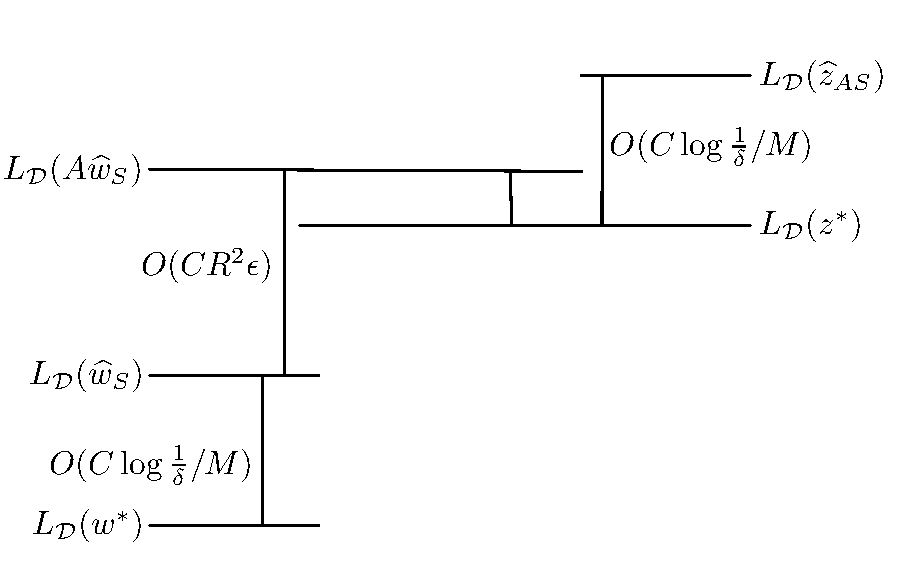
\includegraphics[width=\columnwidth]{bounds_argument_figure.pdf}
    \end{figure}
\end{frame}

\begin{frame}
    \frametitle{RIP for Dot Products}
\end{frame}

\subsection{Extension to Regression}

\begin{frame}
    \frametitle{Support Vector Regression}
\end{frame}

\begin{frame}
    \frametitle{Compressed Learning for Support Vector Machines}
\end{frame}

\subsection{Other Attempted Generalizations}

\begin{frame}
    \frametitle{Attempts to Generalize to other Kernels}
\end{frame}

\begin{frame}
    \frametitle{Attempts to Generalize to Linear Regression}
\end{frame}

\section{Explicit RIP Constructions}

\subsection{}
\begin{frame}
\frametitle{RIP constructions with $m = \tilde{O}(k)$}
Draw a random matrix with entries sampled from $\mathcal{N}(0,1/m)$.

Draw a random matrix with entries sampled from $\left\{+\frac{1}{\sqrt{m}}, -\frac{1}{\sqrt{m}}\right\}$ with Bernoulli parameter $0.5$. 
\end{frame}

\begin{frame}
\frametitle{But...}
\begin{theorem}[\cite{Bandeira12}]
Given a matrix $\Phi$ and parameters $(k,\epsilon)$, certifying whether $\Phi$ is $(k,\epsilon)$-RIP is NP-hard. 
\end{theorem}
\end{frame}

\begin{frame}

\includegraphics[width=4in]{rip.jpg}
\end{frame}


\subsection{Bipartite graph model of measurement}
\begin{frame}
\frametitle{Bipartite graph model of measurement}	
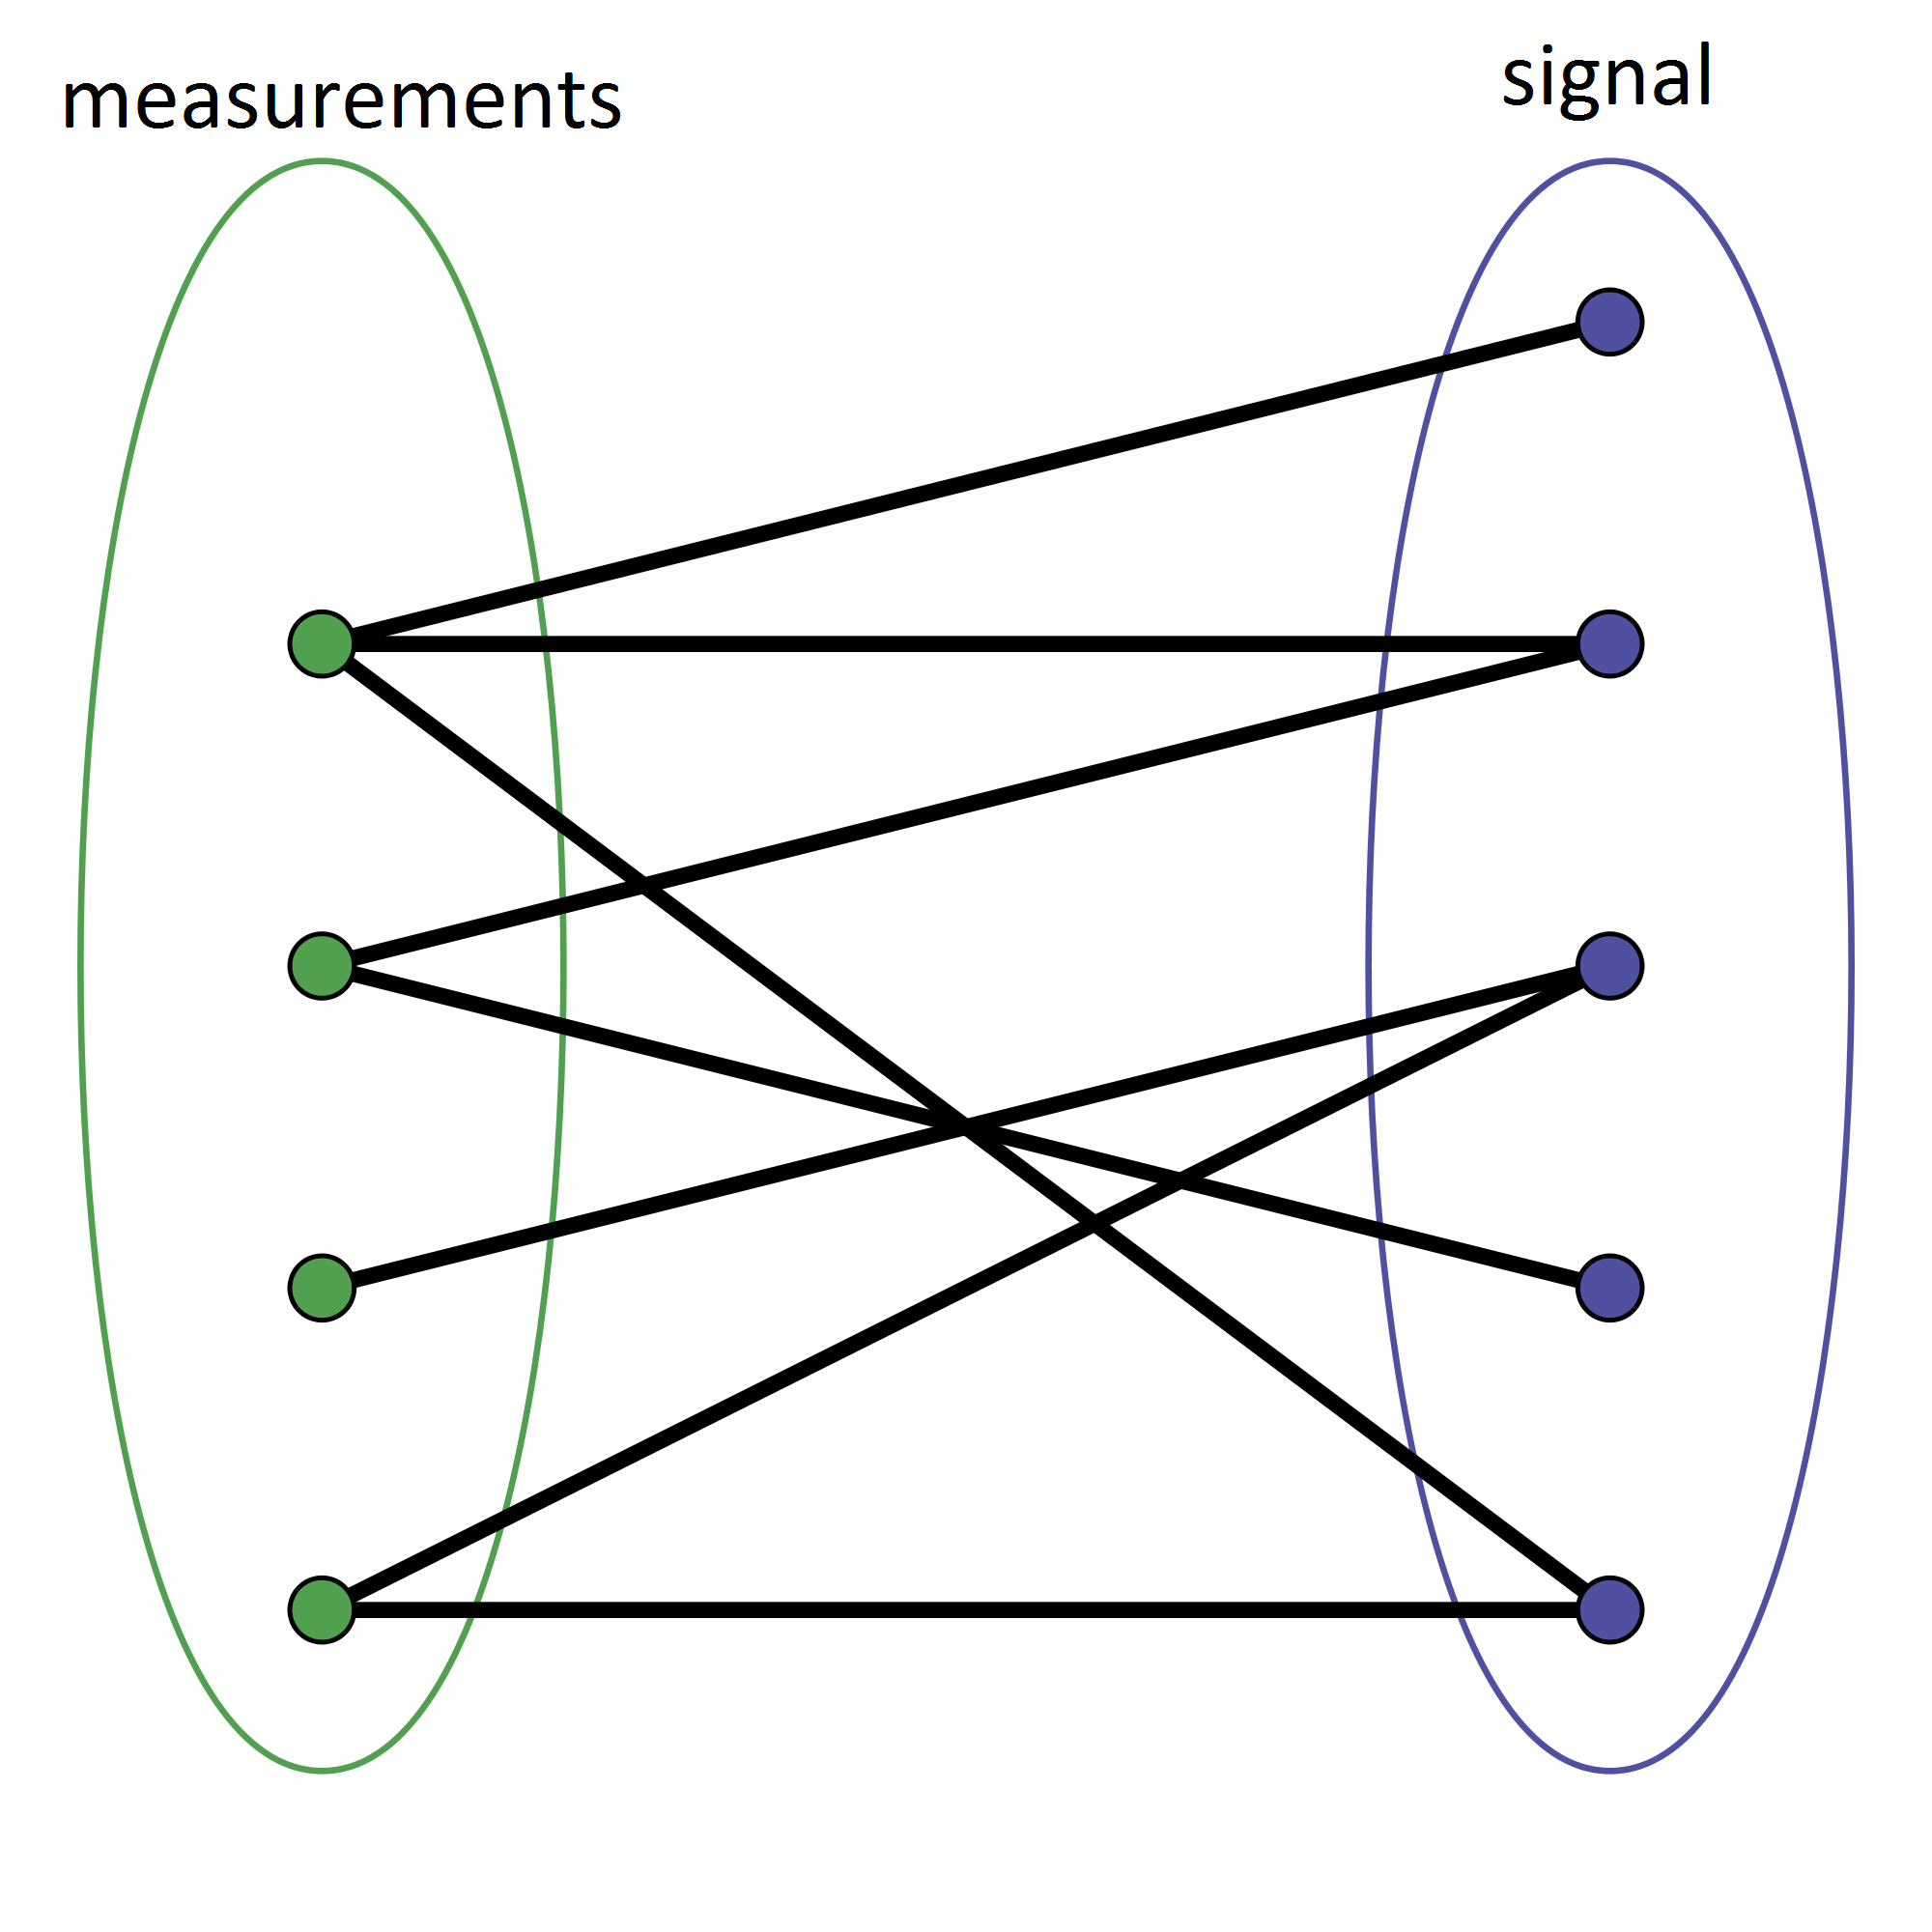
\includegraphics[width=3in]{bpgraph.png}
\end{frame}

\begin{frame}
\frametitle{Expander graphs}

\begin{definition}[Vertex expansion]
	Let $G = (A,B,E)$ be a bipartite graph with left degree $d$. G has $(k,\epsilon)$-vertex expansion if for every subset $X \subset A, |X| \le k$, the set of neighbors $N(A) = \{j \in B \, | \, \exists \, i \in X, (i,j) \in E\}$ has size at least $|N(A)| \ge (1-\epsilon)d|X|$.
\end{definition}

Capture many properties of random graphs, but can be constructed deterministically. 

\end{frame}

\begin{frame}
    \frametitle{Explicit RIP for $\ell_1$-norm}
    \begin{theorem}[\cite{Berinde2008}]
    Let $(A,B,E)$ be a bipartite expander graph with left degree $d$ and with $(k,\epsilon)$-vertex expansion. That is, for all $X \subset A, |X| < k$, then $|N(X)| \le (1-\epsilon)d|X|$. Then the scaled adjacency matrix $\dfrac{1}{d^{1/p}}\Phi$ satisfies the $(p,k,\epsilon)-$RIP property
    
    \[(1-\epsilon)\|x\|_p^2 \le \|\Phi x\|_p^2 \le (1+\epsilon)\|x\|_p^2\]
    for all $k$-sparse $x$ and for $p$ close to $1$. 
	
    \end{theorem}	

\end{frame}

\begin{frame}
\frametitle{Extension to $\ell_2$-norm}
There's a lower bound for the $\ell_2$ norm: a $\{0,1\}$ matrix which satisfies the RIP property must have $m = \Omega(k^2)$. 

Possible way around the lower bound: use multigraphs. $\Phi_{ij} = \#$ of edges between $i$ and $j$. 

Generalize the lower bound in terms of an inequality involving the $\ell_1,\ell_2$ norms of the columns?

\end{frame}

%
%\subsection{Nonnegative RIP matrices}
\begin{frame}
\frametitle{A more modest question}
Are cancellations in sign necessary for the $\ell_2$ norm?

Can RIP matrices with $m = \tilde{O}(k)$ can be constructed using only nonnegative entries?
 
\end{frame}

\subsection{Poisson Random Matrices}
\begin{frame}
    \frametitle{Poisson Random Matrices}
    Given $a,b \sim \text{Pois}(\lambda)$, $\mathbb{E}[ab] = \lambda^2$ and $\mathbb{E}[a^2] = \lambda$.
    For $\lambda << 1$, this property seems almost as good as $\mathbb{E}[ab] = 0$ for Gaussian random variables. 
    
    \begin{Lemma}
    	
    Given a matrix $\Phi$ where $\Phi_{ij} \sim \text{Pois}(\lambda)$, we have
    \[\|x\|_2^2 \le \mathbb{E}\left[\left\|\frac{1}{m\lambda}\Phi x\right\|_2^2\right] \le (1+\lambda k)\|x\|_2^2\]	
    \end{Lemma}

\end{frame}

\begin{frame}[t,allowframebreaks]{}
\frametitle{References}

\bibliographystyle{plainnat}
\bibliography{biblio}
\end{frame}


\end{document}

